\section{Design}

This section outlines the overall design of our project, including the architecture, technology stack, and deployment process. We also discuss the cloud provider, infrastructure, version control, and continuous integration/continuous delivery (CI/CD) practices employed.

\subsection{Overview}

Our system comprises three main layers: the Front-end UI layer, the API layer, and the Back-end layer. The front-end UI layer is the user-facing component of our application and is hosted as a web application. It provides a graphical user interface that enables users to interact with the system and access the information they need.

As you can see in \autoref{fig:sequence-diagram}, the API layer is hosted on Azure and is implemented using .NET. It serves as the communication interface between the Front-end UI layer and the Back-end layer. The API layer receives requests from the Front-end UI layer, processes them, and sends them to the Back-end layer for data retrieval and processing. The API layer also handles authentication and authorization, ensuring that users only have access to the data they are authorized to view.

The Back-end layer is hosted on AWS and is responsible for storing and processing data. It comprises a variety of services and components, including databases, storage systems, and compute resources. The Back-end layer receives requests from the API layer, processes them, and sends the results back to the API layer for transmission to the Front-end UI layer.

By splitting our system into these three layers, we are able to achieve better scalability, maintainability, and fault tolerance. The separation of concerns also makes it easier to add new features and functionality to the system over time.

\begin{figure}[htp]
    \centering
    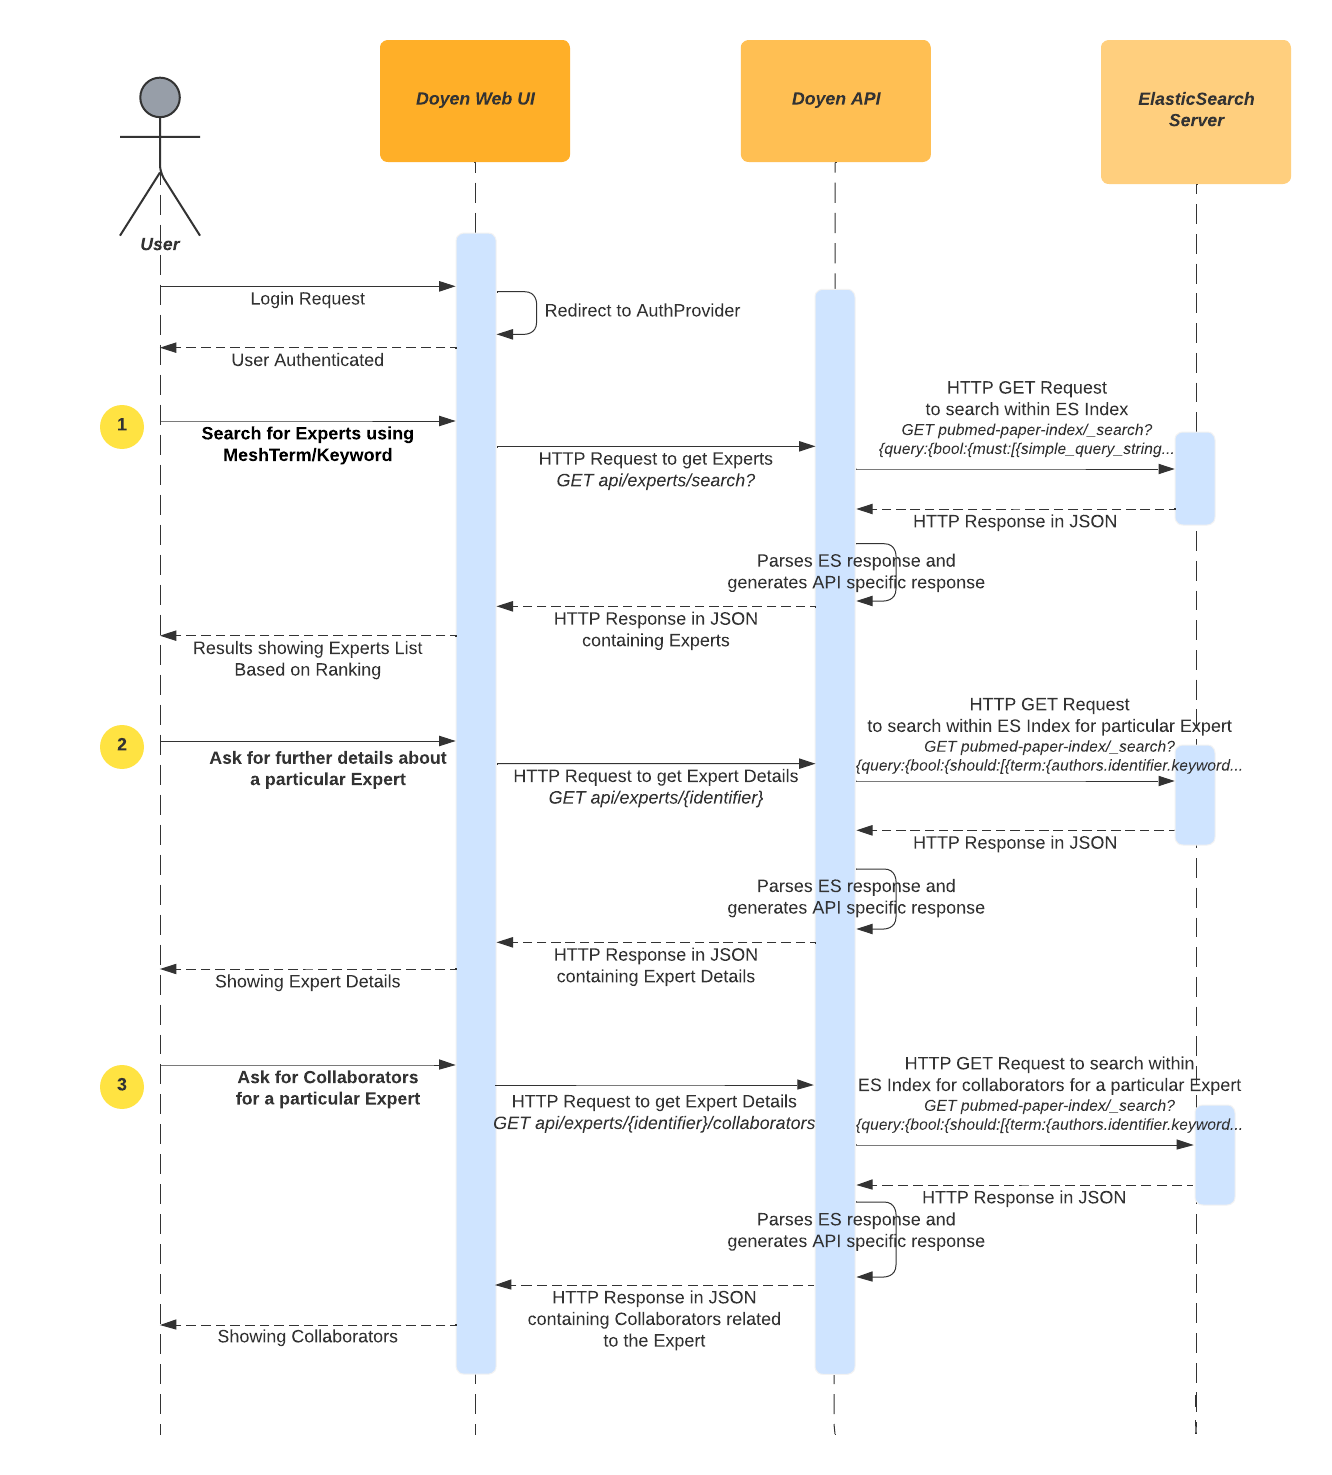
\includegraphics[width=\textwidth]{Images/SequenceDiagram_GetExperts.png}
    \caption{End-to-end flow - Sequence Diagram}
    \label{fig:sequence-diagram}
\end{figure}


\subsection{Front-End}

For the front-end of our application, we chose to implement the client using Next.js 13, a popular and efficient React framework for building user interfaces. Next.js allows us to create modular and reusable components, enhancing our application's development speed and maintainability.

In addition to Next.js, we utilized Tailwind CSS as our front-end styling framework. Tailwind is a highly customizable, low-level CSS framework that promotes a utility-first approach to styling. This choice enabled us to quickly build consistent, responsive, and performant user interfaces with minimal CSS overhead.

\subsection{Back-End}

Our back-end services are hosted on Amazon Web Services (AWS) EC2 instance and Azure. AWS EC2 allows users to launch Virtual Machines on the Amazon Cloud infrastructure with various workloads and application combinations. This choice allows us to focus on our application's functionality while AWS handles the scaling and maintenance of the underlying infrastructure. The API Gateway is the entry point for our back-end services, providing a fully managed service for creating, publishing, and maintaining secure APIs.

We implemented our data ingestion layer  using PySpark, a Python library for Apache Spark. PySpark allows us to process large-scale data in parallel, enabling efficient data manipulation and transformation. Furthermore, we built our ingestion pipeline using Python.

The back-end service API layer is implemented in .Net using C\# and hosted on Microsoft Azure Cloud. This combination enables us to build scalable and maintainable server-side applications while leveraging the vast ecosystem of Microsoft .Net libraries and tools.

\subsection{Ingestion Pipeline}

Our system has an ingestion pipeline workflow, shown in \autoref{fig:ingestion-flow}, which automatically downloads baseline data from the PubMed FTP server and processes it. The processed data is then stored in an Elasticsearch instance, which is hosted on an EC2 instance inside a Docker container. The ingestion pipeline is also located on the same EC2 instance and runs on demand.

To keep the Elasticsearch index up-to-date, we have implemented a daily cron job that downloads the daily update PubMed file from the Ftp server and runs the same ingestion pipeline. This ensures that the Elasticsearch index is always up-to-date and reflects the latest changes in the Pubmed database.

By automating the data ingestion process and implementing the daily cron job, we have reduced the manual effort required to update the Elasticsearch index, minimized the risk of errors and inconsistencies, and ensured that our system is always working with the most up-to-date data.

\begin{figure}[htp]
    \centering
    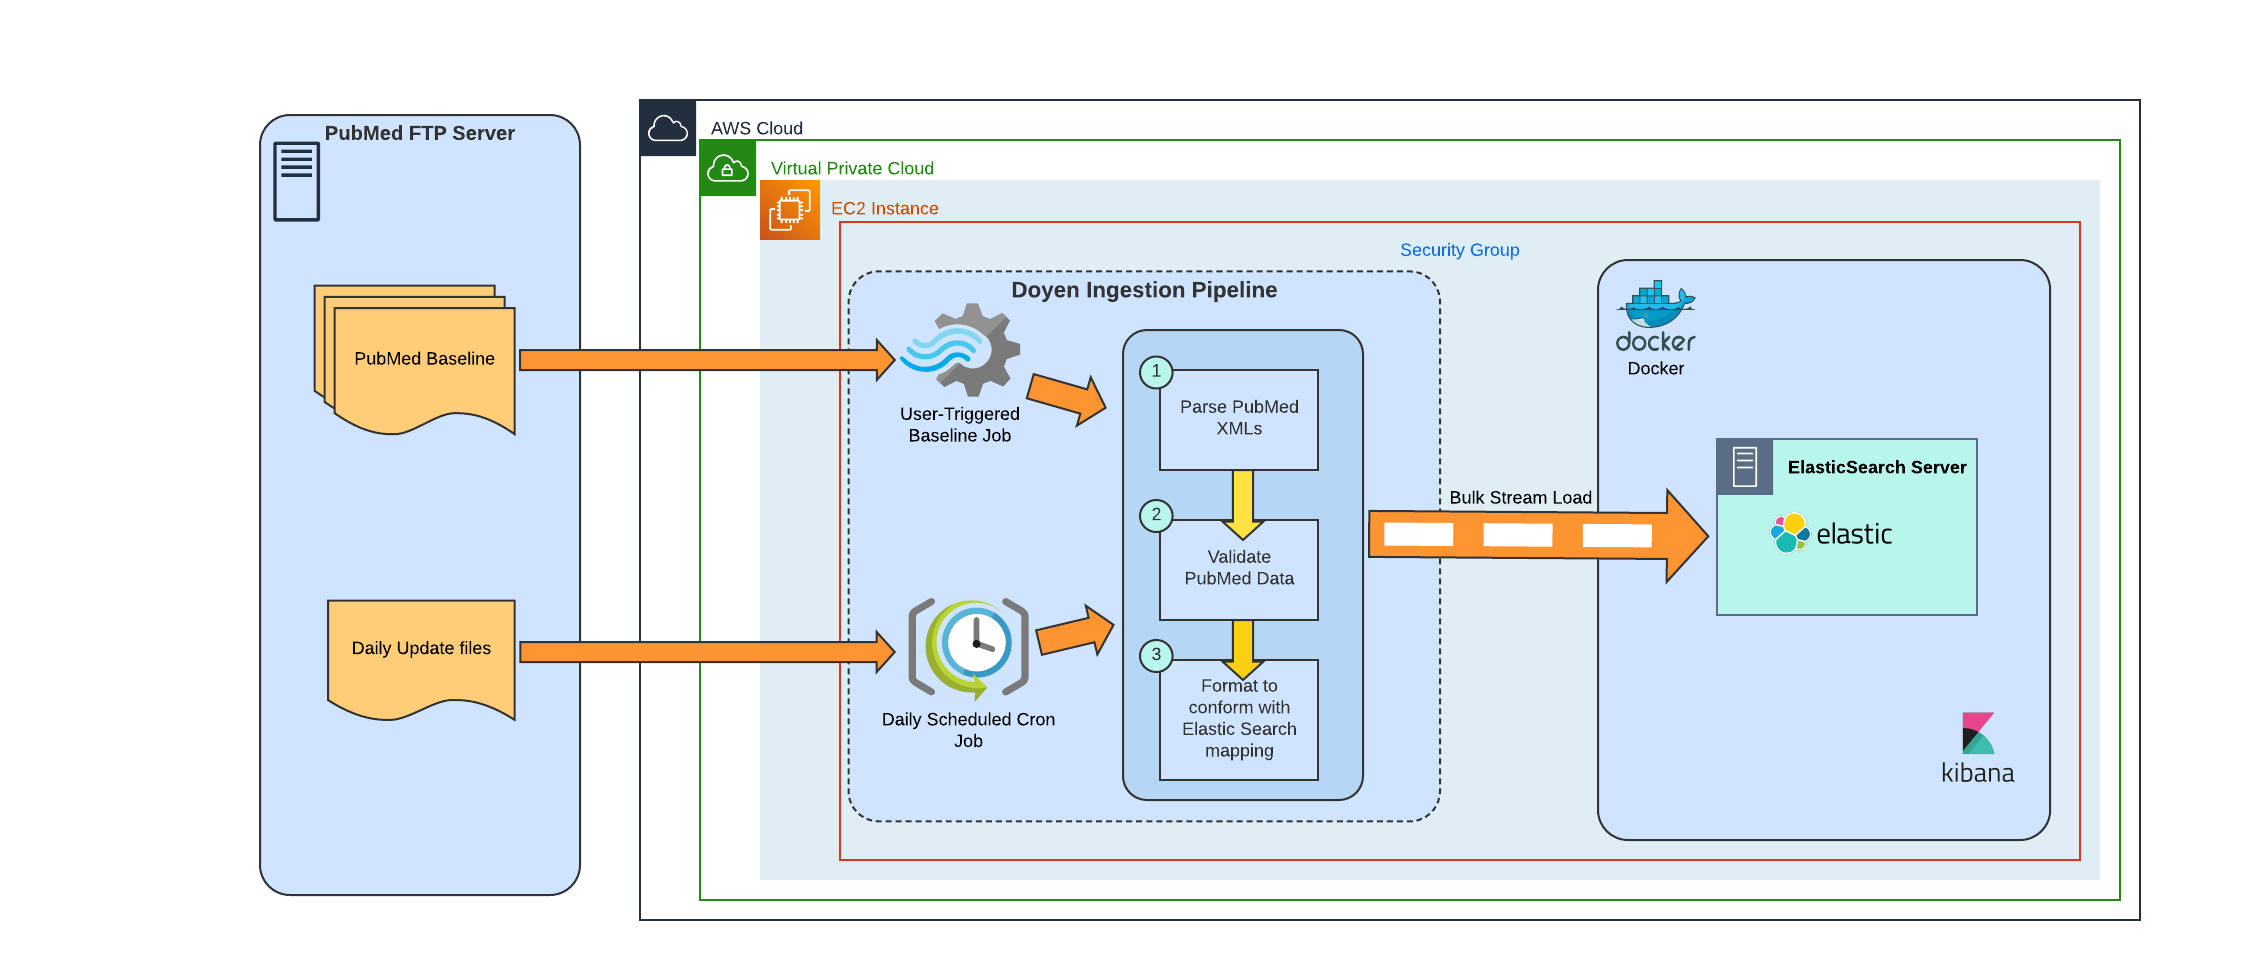
\includegraphics[width=\textwidth]{Images/Ingestion Pipeline flow.png}
    \caption{Ingestion Pipeline Flow}
    \label{fig:ingestion-flow}
\end{figure}


In \autoref{fig:ingestion}, you can see the Ingestion Pipeline comprises several classes, with the main entry point being the PubmedProcessor class. This class contains functions to create the Elasticsearch PubMed index and ingest files, utilizing the Elasticsearch and NihFtpClient libraries.

\begin{figure}[htp]
    \centering
    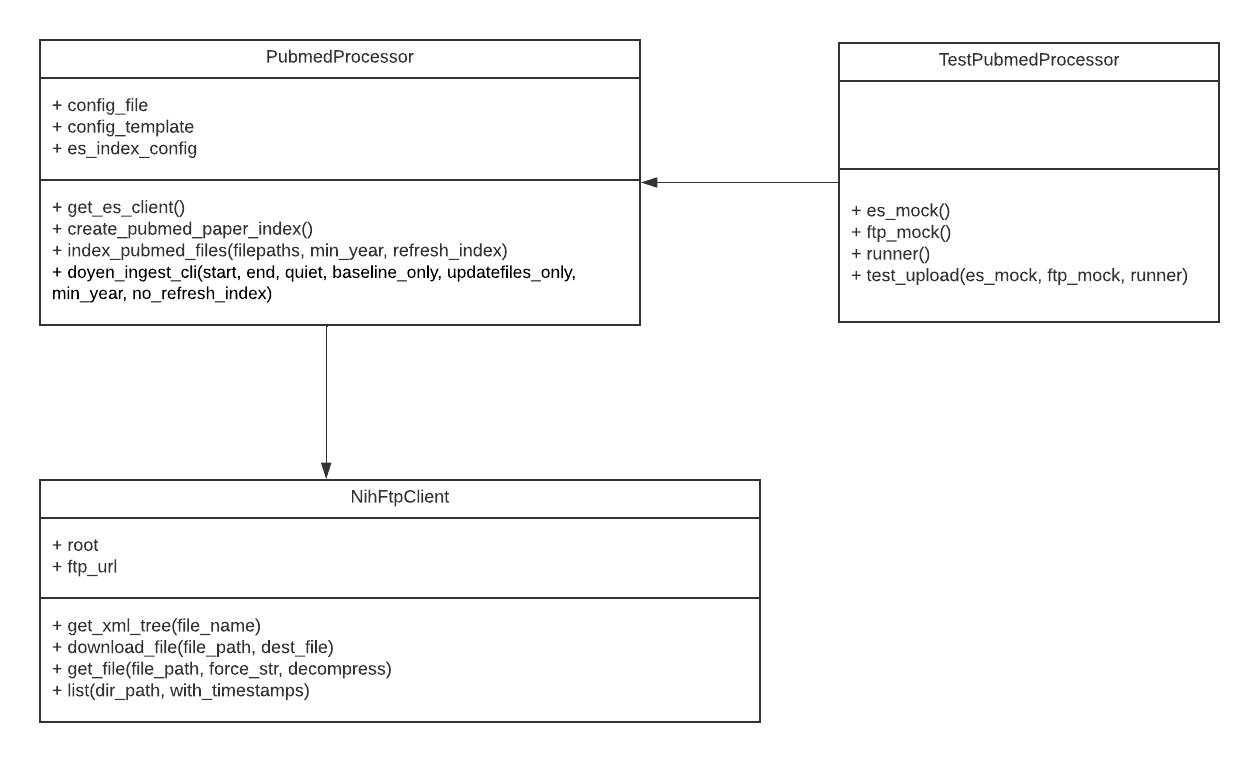
\includegraphics[width=\textwidth]{Images/IngestionPipeline_ClassDiagram.png}
    \caption{Ingestion Pipeline Model - Class Diagram}
    \label{fig:ingestion}
\end{figure}



\subsection{API Layer}

The API layer, shown in \autoref{fig:api-layer} is a crucial component that facilitates communication between the front-end and back-end. It serves as the primary interface for the front-end to interact with the back-end services. The API layer is responsible for managing and processing incoming requests from the front-end and sending them to the Elasticsearch Server for data retrieval. It executes queries against the server to retrieve the desired data and refines and translates it into a format that is easily digestible for the front-end.

Apart from basic search queries, the API layer is also responsible for running advanced queries, such as aggregated queries, to extract expert-related information like collaborators, research interests, and more. The API layer plays a vital role in providing a seamless user experience, ensuring that data is processed and delivered efficiently and accurately. It also allows the system to be extensible, bringing in additional or changing data sources to supplement current data  without breaking the interface to the UI.


\begin{figure}[htp]
    \centering
    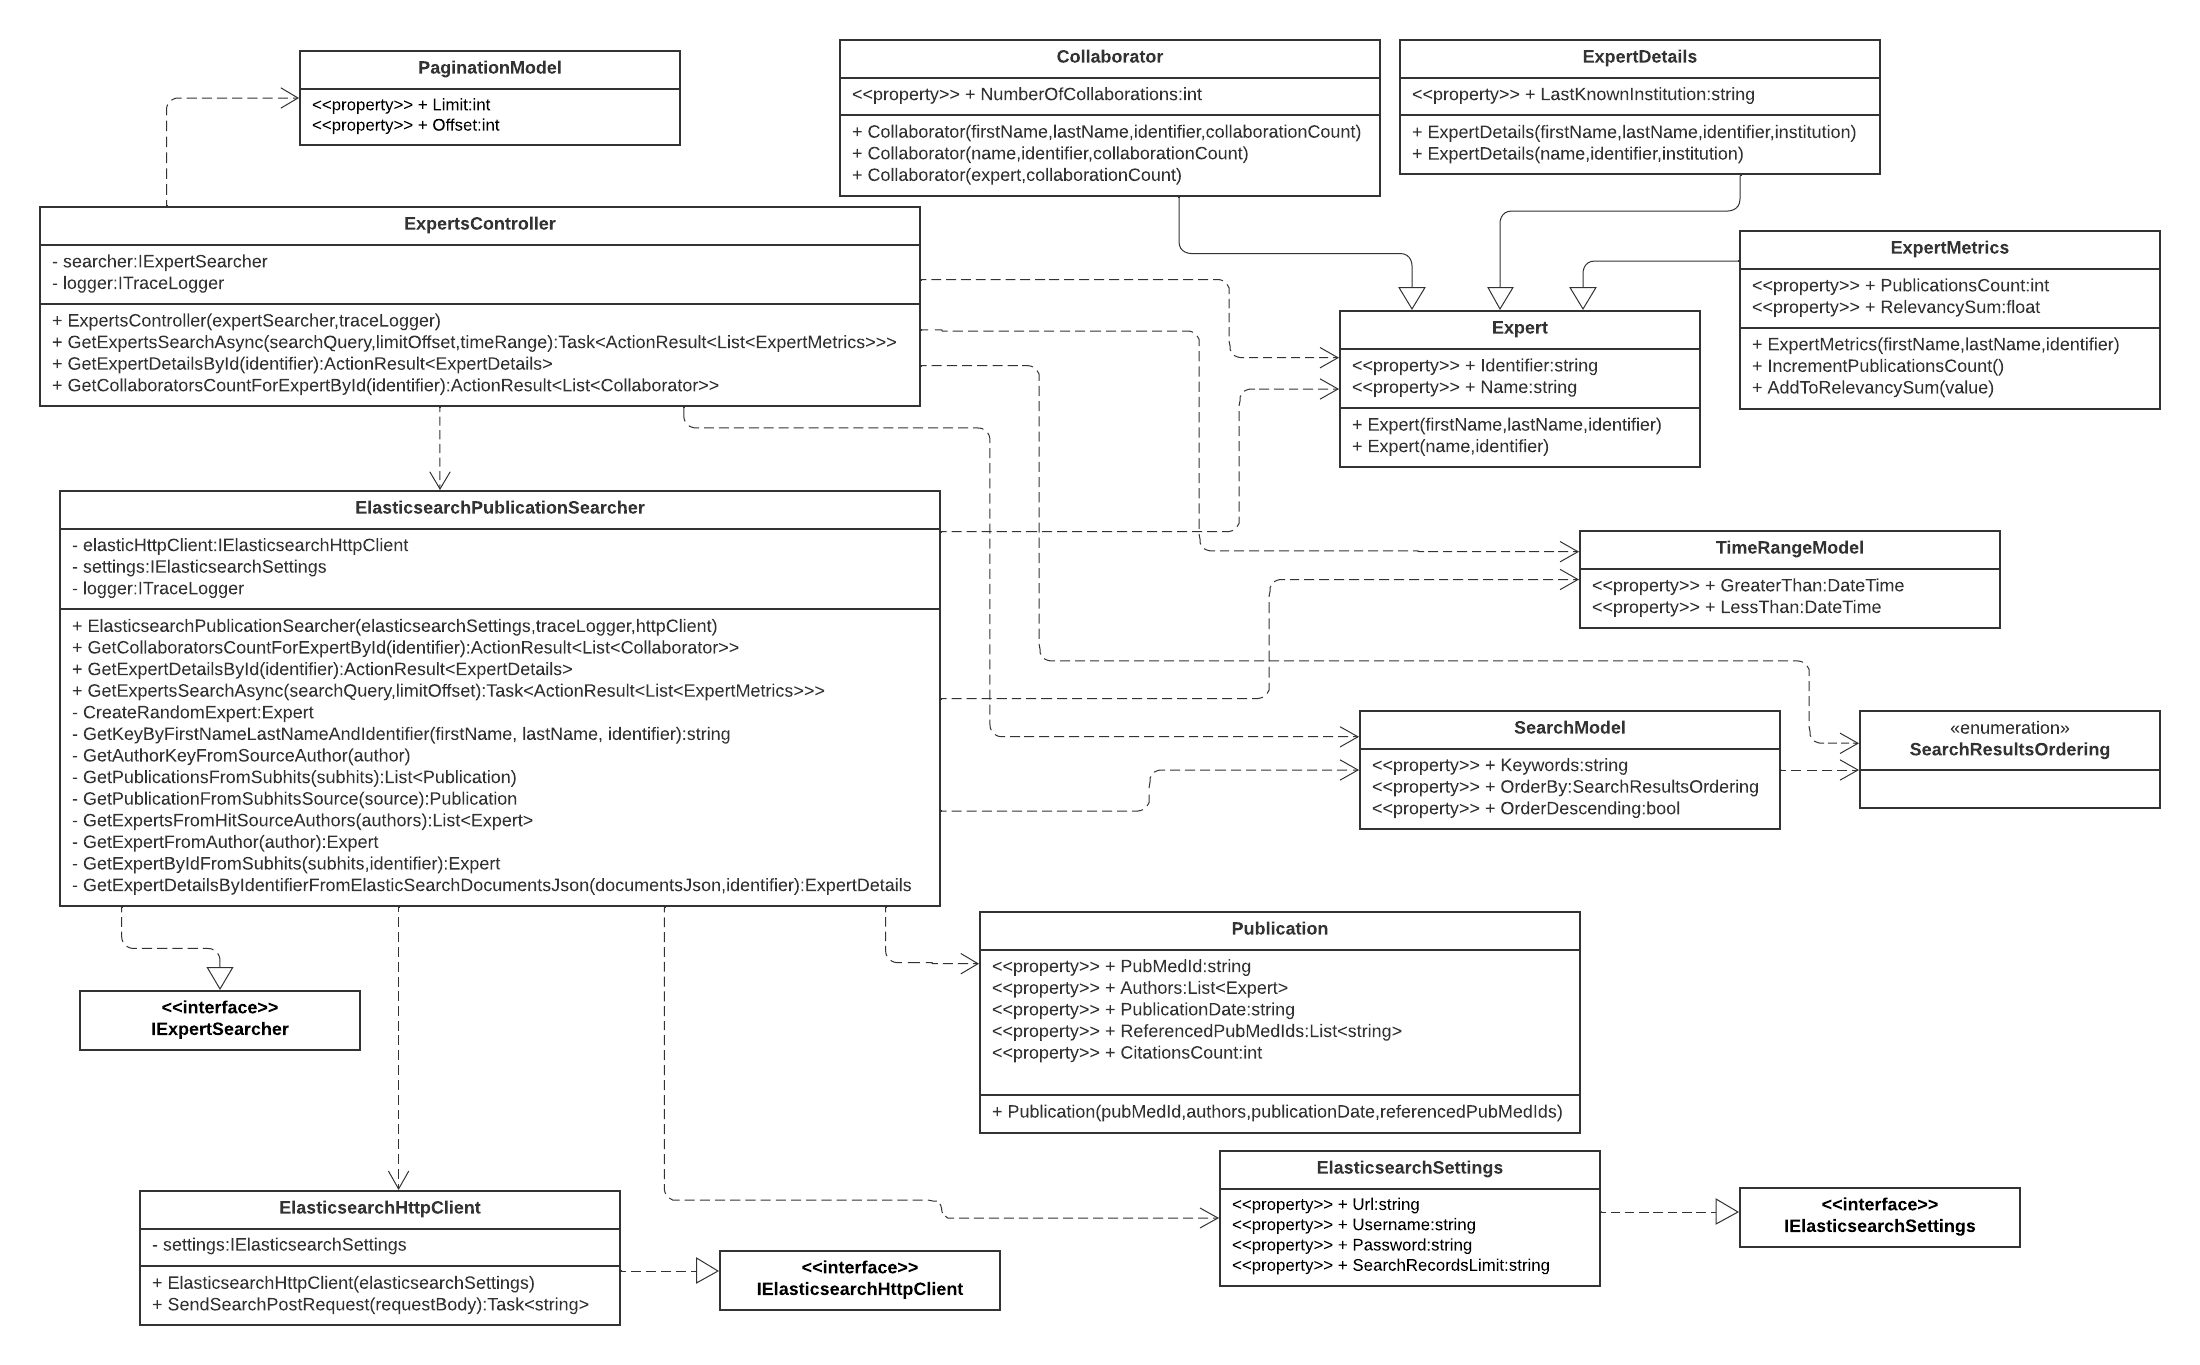
\includegraphics[width=\textwidth]{Images/API_ClassDiagram.png}
    \caption{API Layer - Class Diagram}
    \label{fig:api-layer}
\end{figure}

\subsection{Data Management}

Our primary data is hosted and searched using Elasticsearch, a powerful and flexible search and analytics engine. Elasticsearch allows us to store, search, and analyze large volumes of data quickly and in near real-time.

Additionally, we store extra data in Amazon Simple Storage Service (S3), a highly-scalable and durable object storage service. Amazon S3 provides a cost-effective, secure solution for storing and retrieving extensive data.

\subsection{Cloud Provider}

For our cloud provider, we selected Amazon Web Services (AWS). AWS offers a comprehensive suite of tools and services to help us build, deploy, and manage our application effectively and securely.

\subsection{Infrastructure}

As previously mentioned, our primary data is hosted in Elasticsearch. To manage our resource deployments, we utilized AWS CloudFormation,  enabling us to create and manage a collection of AWS resources using templates. This approach helped streamline infrastructure management and ensure a consistent and reproducible environment. The overall architecture is shown in \autoref{fig:architecture}.

We also use AWS CloudFront, a global content delivery network (CDN) service, to serve our front end. CloudFront accelerates the delivery of our application's assets by caching and distributing them across a network of edge locations, improving the overall user experience.
Our back-end is hosted on AWS Lambda and served through Amazon API Gateway, as discussed in section 2.2.

\begin{figure}[htp]
    \centering
    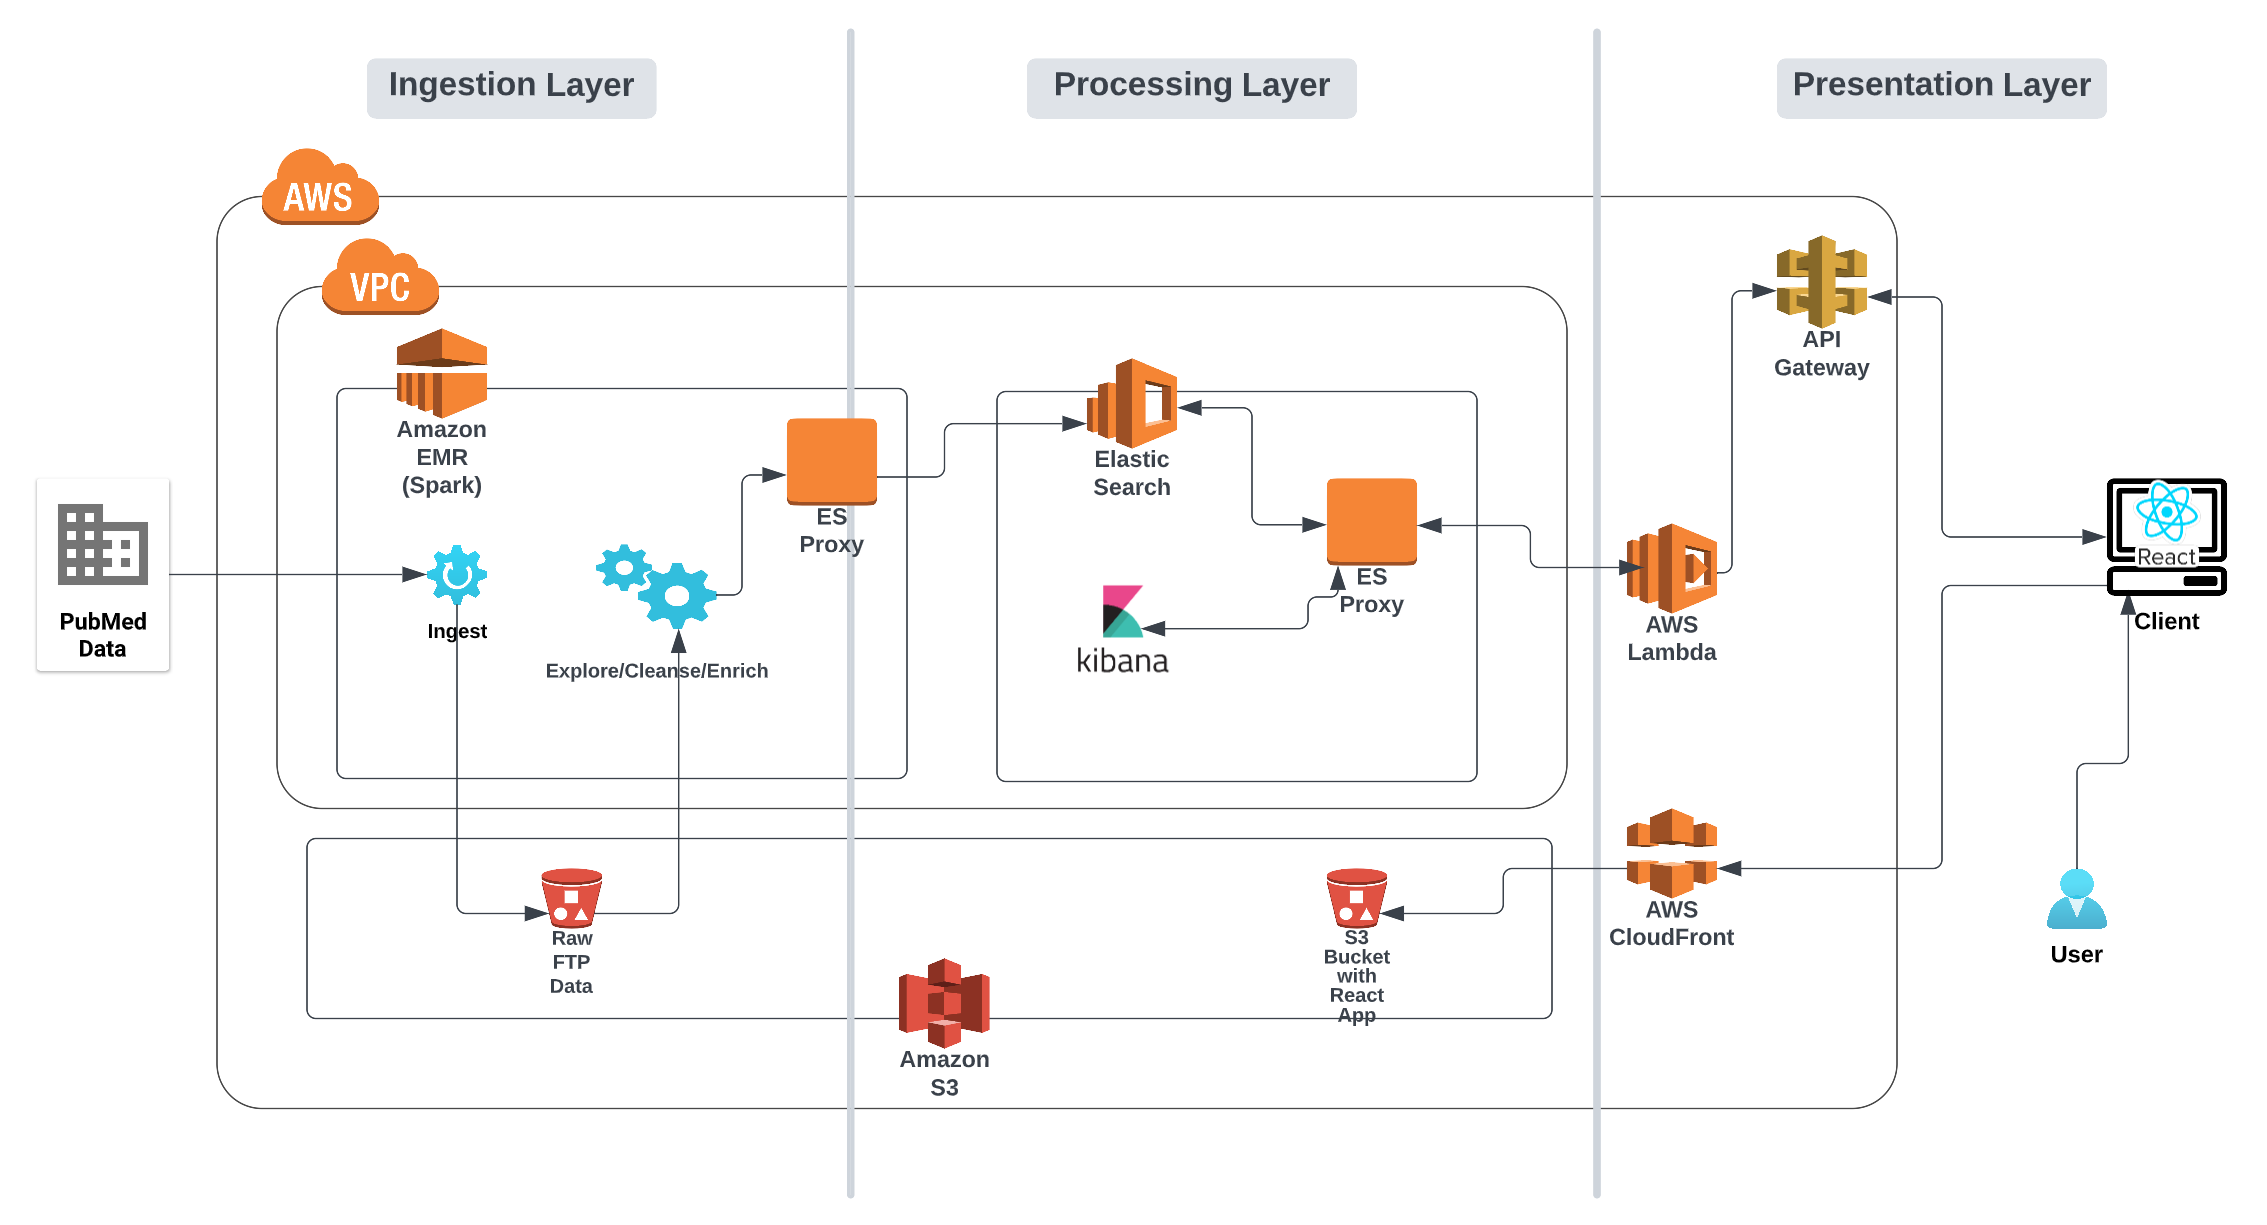
\includegraphics[width=\textwidth]{Images/Doyen High-Level Architecture Diagram.png}
    \caption{The Doyen Architecture}
    \label{fig:architecture}
\end{figure}

\subsection{Version Control and CI/CD}

We used GitHub for version control, allowing us to manage our codebase effectively, track changes, and collaborate efficiently. GitHub also implements our continuous integration/continuous delivery (CI/CD) pipeline. This pipeline automates the process of building, testing, and deploying our application, ensuring we maintain a high code quality and consistency throughout the project's lifecycle. By implementing a CI/CD pipeline, we can detect and address issues early, reduce manual intervention, and streamline the delivery of new features and bug fixes.

In conclusion, our project's design incorporates modern and scalable technologies to ensure a robust and maintainable application. Our choice of AWS as a cloud provider, combined with implementing CloudFormation, CloudFront, and a CI/CD pipeline using GitHub, allows us to streamline our infrastructure management and ensure a consistent and reproducible environment for our application. By utilizing Next.js, Tailwind CSS, Elasticsearch, AWS Lambda, and API Gateway, we built an efficient and responsive front-end and a reliable and scalable back-end and effectively manage our data.